\documentclass{beamer}

\usepackage[T1]{fontenc}
\usepackage[english]{babel}
\usepackage[utf8]{inputenc}
\usepackage{newunicodechar}
% !TEX spellcheck = en_US

\usetheme[progressbar=frametitle]{metropolis}
\usepackage{appendixnumberbeamer}
\usepackage[percent]{overpic}
\usepackage{multicol}
\usepackage{subfigure}
\usepackage{graphicx}

\title{
	Two-step multi-spectral registration via key-point detector and gradient similarity. \\
	\vspace{1em}
	Application to agronomic scenes for proxy-sensing.
}
\date{\today}
\author{
	Vayssade Jehan-Antoine \\
	\tiny \url{jehan-antoine.vayssade@inra.fr}
}
\institute{
	AgroSup Dijon, Pole GestAd in Precision Farming group, France  \\
	Gawain Jones, Jean-Noël Paoli, Christelle Gee
}

\definecolor{OliveGreen}{HTML}{556B2F}

\begin{document}

	\maketitle
	
	\section{Introduction}
	
		\begin{frame}{Working environment}
			New consumer and environmental requirements
			
			\vspace{-0.5em}
			\begin{itemize}
				\small
				\item Reduction of plant protection products
				\item Government plans Ecophyto (I, II, II+)
			\end{itemize}
			
			\begin{figure}
				\centering
				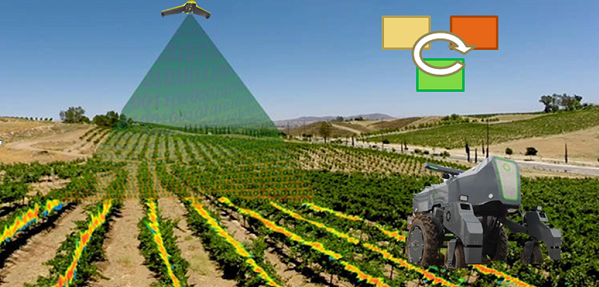
\includegraphics[width=0.5\linewidth]{roseau}
				\label{fig:roseau}
			\end{figure}
			
			How can these new requirements be met ?
			
			\vspace{-0.5em}
			\begin{itemize}
				\small
				\item Localized control of weeds by imaging 
				\item Agricultural Robotics (Pumagri / SITIA)
			\end{itemize}
		\end{frame}
	
		\begin{frame}{Working environment}
			\begin{figure}
				\centering
				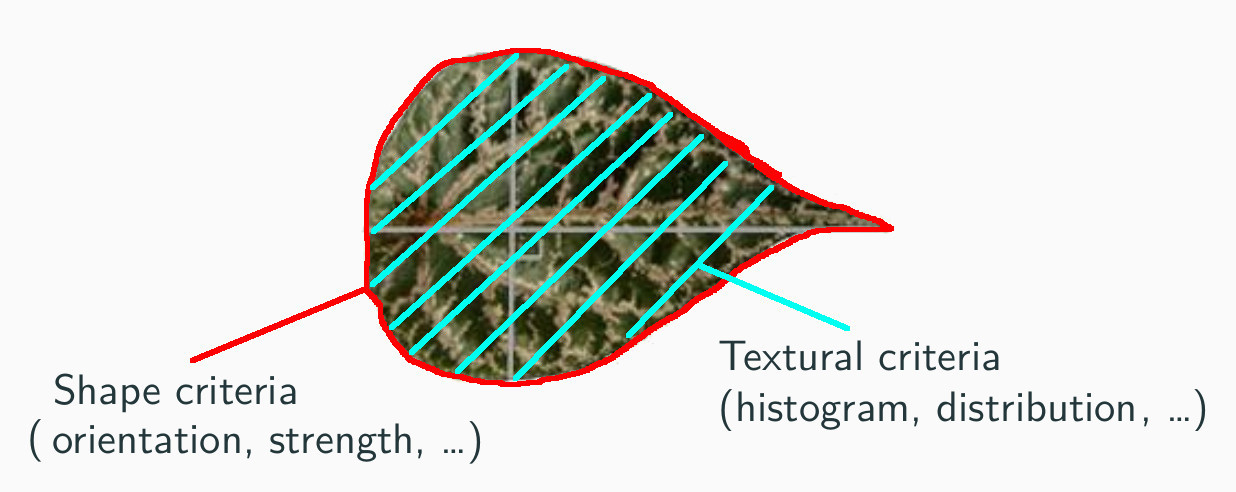
\includegraphics[width=\linewidth]{leaf}
				\caption{We search for criteria that can discriminate weeds and crops}
			\end{figure}
		\end{frame}
	
		\begin{frame}{Main Question}
			In precision farming, major mistakes are still done in image registration.
			There is no broad study of :
			
			\begin{itemize}
				\item the best spectral band to use as reference
				\item the most adapted key-points extractor algorithms
			\end{itemize}
		\end{frame}
	
		\begin{frame}{Focuses}
			This paper focuses on these two points and defines :
			\begin{itemize}
				\item a benchmark of different key-points detectors (time/number)
				\item a benchmark for each spectral reference.
			\end{itemize}
		\end{frame}
	
		\begin{frame}{Material}
			\begin{figure}
				\centering
				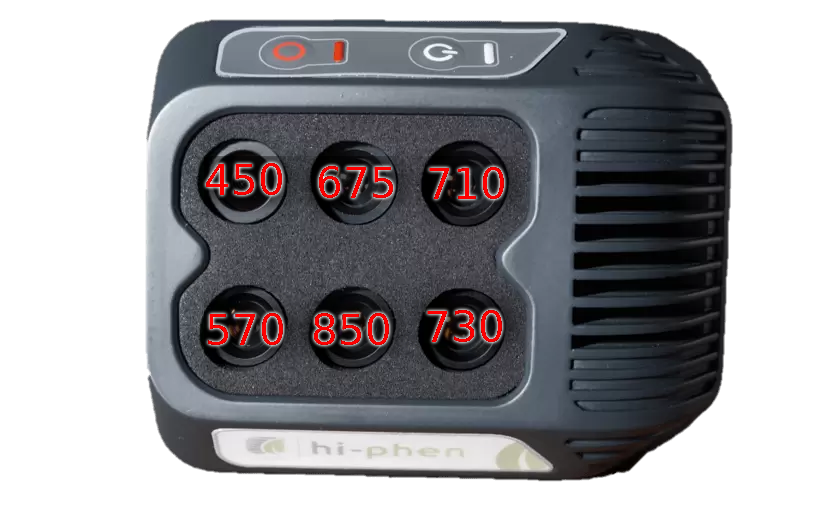
\includegraphics[height=3cm]{../figures/airphen-detail4.png}
				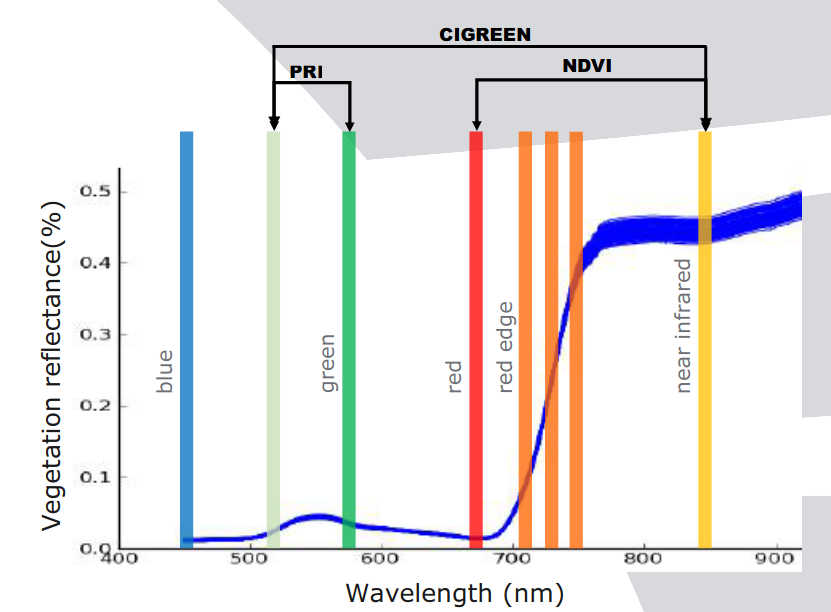
\includegraphics[height=3cm]{wavelengths.png}
				\caption{AIRPHEN camera}
			\end{figure}
			\begin{itemize}
				\item interferential filters centered at {\small 450/570/675/710/730/850 nm}
				\item small width of each wavelengths (10 FWHM)
				\item focal lens is 8 mm for all wavelengths
				\item raw resolution $1280 \times 960$ px with 12 bit of precision.
				\item internal GPS antenna (3D position)
			\end{itemize}
		\end{frame}
	
		\begin{frame}{Data}
			Two datasets were taken, one for calibration, one for evaluation.
			\begin{figure}
				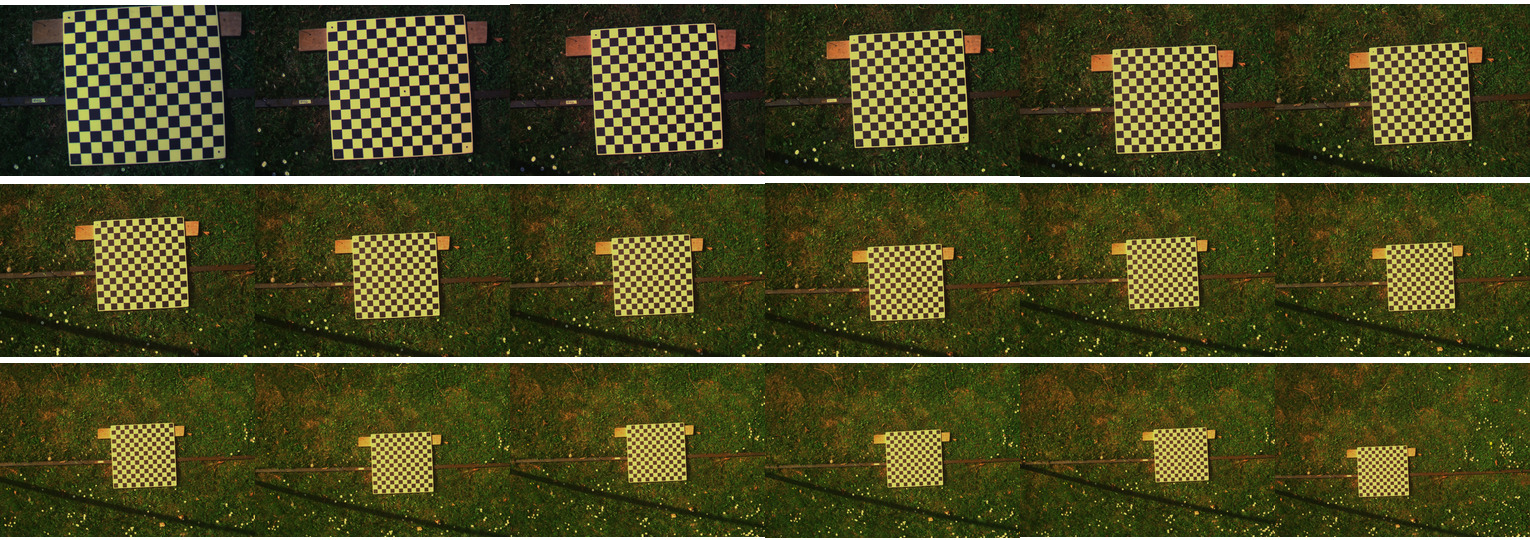
\includegraphics[width=\linewidth]{../figures/calibration-height.jpg}
				\caption{false color reconstruction of each acquisition height (18) for calibration dataset, from 1.2 to 5 meters.}
			\end{figure}
		\end{frame}
	
	\section{Methods}
	
		\begin{frame}{Two steps : rough and full}
			\begin{figure}
				\centering
				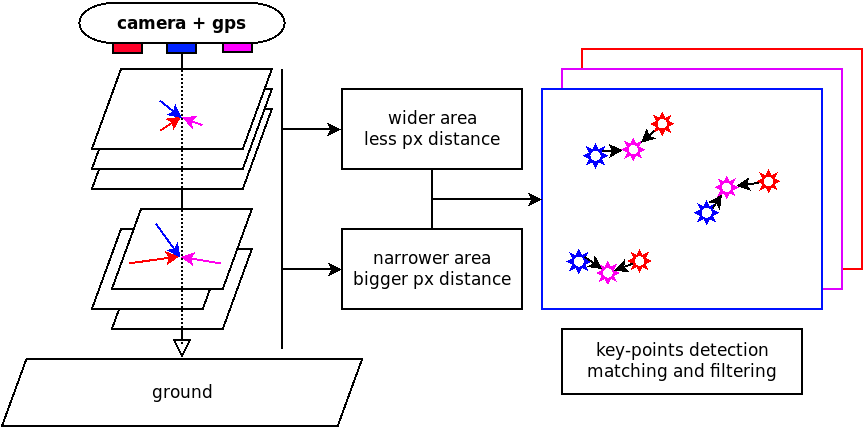
\includegraphics[width=\linewidth]{Diagram1}
				\caption{Rough registration through calibration and GPS (left) and refinement using key-point (right)}
				\label{fig:diagram1}
			\end{figure}
		\end{frame}
	
	
		\begin{frame}{Affine Calibration, translation part}
			\begin{figure}
				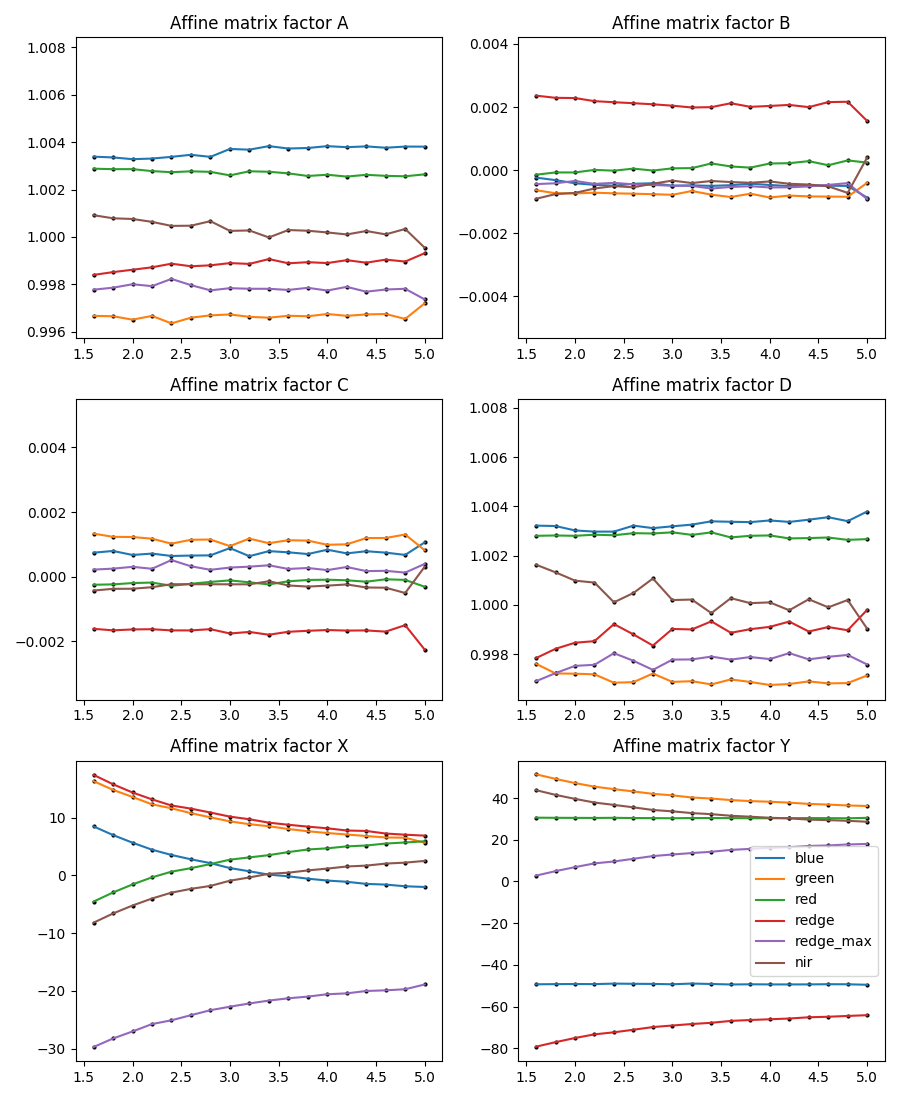
\includegraphics[width=0.7\linewidth]{../figures/affine-translation-height.png}
				\caption{Translation factors from detected chessboard to ``virtual'' center chessboard at each acquisition height}
			\end{figure}
		\end{frame}

		\begin{frame}{Affine Calibration, rotation\&scale part}
			\begin{figure}
				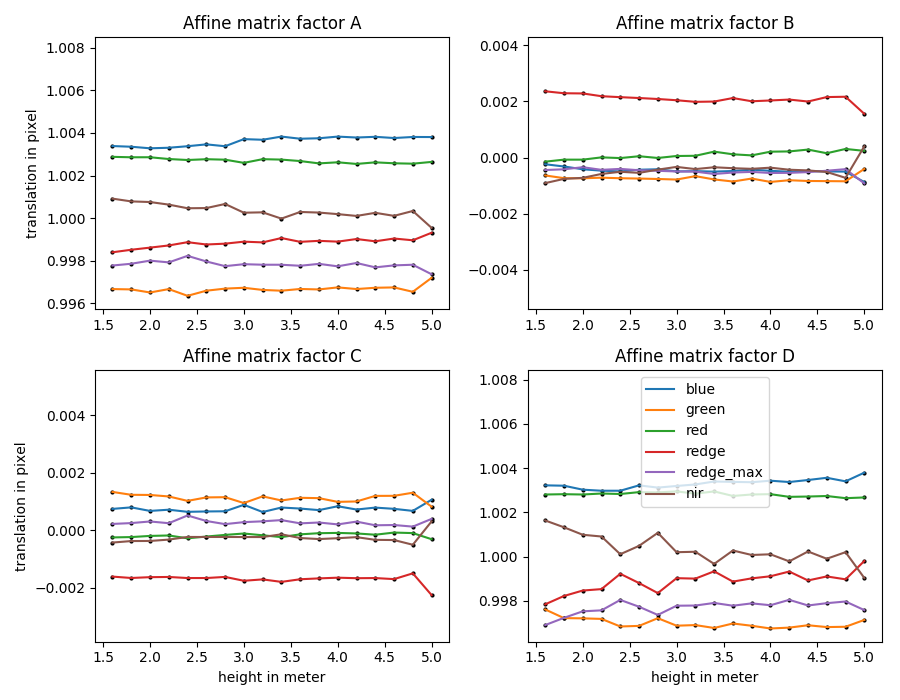
\includegraphics[width=0.7\linewidth]{../figures/affine-rotation-height.png}
				\caption{Rotation and scale factors from detected chessboard to ``virtual'' center chessboard at each acquisition height (precision depends on height but we can notice that these factors are likely invariant)}
			\end{figure}
		\end{frame}
	
		\begin{frame}{Affine Correction}
			From that calibration an affine matrix model is built:
			
			\begin{itemize}
				\item For $A,B,C,D$ the values at the most accurate height are used
				\item For $X,Y$ factors an equation is fitted for each spectral band \footnote{Levenberg-Marquardt with linear least squiss regression}
				\begin{itemize}
					\item $t = \alpha h^3 + \beta h^2 + \theta h + \gamma$
				\end{itemize}
				\item We use the height from the GPS to get the nearest correction
				\item We crop all images to remove the uncovered area
			\end{itemize}
		
			%Each spectral band is warped using the corresponding affine transformation built from the height given by the GPS.
			%And a crop is applied to remove uncovered area.
		\end{frame}
	
	\section{Methods : Perspective correction via key-points detector (refinement)}
	
		\begin{frame}{Gradient transform for key-points detection}
			\begin{figure}
				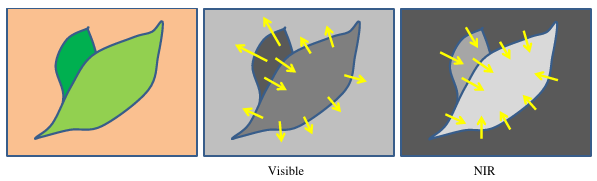
\includegraphics[width=0.7\linewidth]{../figures/contrast-inversion.png}
			\end{figure}
		
			To optimize the search of specific key-points such as gradient breaks,
			each spectral band is transformed :
			\begin{itemize}
				\item normalization using Gaussian blur $I/(G+1)*255$ 
				\item gradient is computed with the sum of absolute Sharr filter
				\item normalization using CLAHE to locally improve their intensity
			\end{itemize}
		\end{frame}
	
		\begin{frame}{Key-points detectors (9)}
			\begin{itemize}
				\item {\color{orange}{(ORB) Oriented FAST and Rotated BRIEF}}
				\item (AKAZE) Fast explicit diffusion for accelerated features in nonlinear scale spaces
				\item {\color{orange}{(KAZE) A novel multi-scale 2D feature detection and description algorithm in nonlinear scale spaces}}
				\item (BRISK) Binary robust invariant scalable key-points
				\item (AGAST) Adaptive and generic corner detection based on the accelerated segment test
				\item (MSER) maximally stable extremal regions
				\item (SURF) Speed-Up Robust Features
				\item (FAST) FAST Algorithm for Corner Detection
				\item {\color{purple}{(GFTT) Good Features To Track}}
			\end{itemize}
		\end{frame}
	
		\begin{frame}{Perspective correction via Keypoint}
			\begin{figure}
				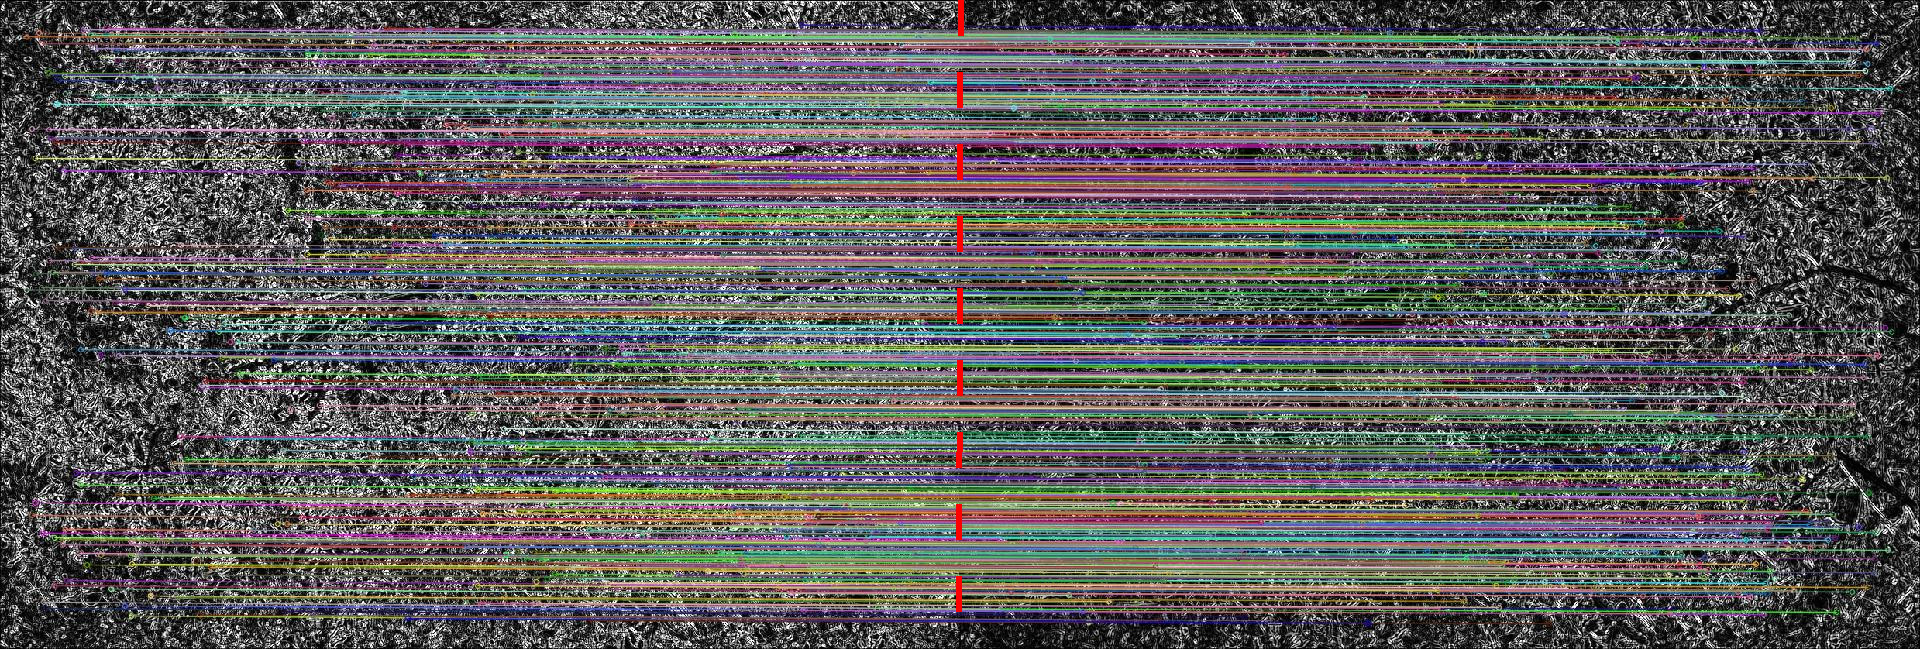
\includegraphics[width=\linewidth]{../figures/prespective-feature-matching}
				\caption{Bruteforce key-points matching in normalized gradient and filtering (reference 570nm left \& 850nm right) using GFTT1}
			\end{figure}
		
			\begin{itemize}
				\item detection inside the normalized gradient
				\item matching using texture properties of the gradient
				\item filtering all matches by bounding them (distance/angle)
			\end{itemize}
		\end{frame}
	
	\section{Results}
	
		\begin{frame}{Results : benchmark of key-points extractors}
			\begin{figure}
				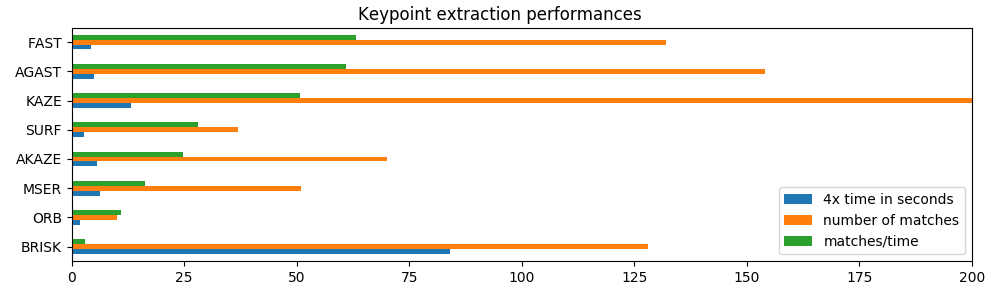
\includegraphics[width=\linewidth]{../figures/comparaison-keypoint-performances}
				\caption{Performances of different key-points detectors}
			\end{figure}
			\vspace{-1em}
			\begin{itemize}
				\item number of matches $\rightarrow$ precision
				\item time $\rightarrow$ lower is better
			\end{itemize}
		\end{frame}
	
		\begin{frame}{Results : benchmark of spectral reference}
			\begin{figure}
				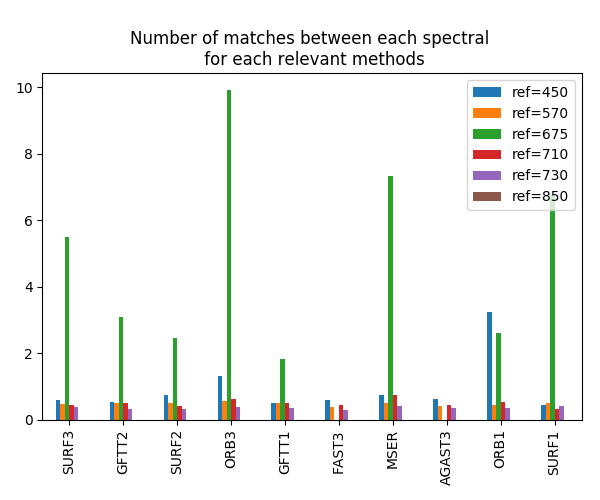
\includegraphics[width=0.6\linewidth]{../figures/comparaison-keypoint-matching-reference-merged.png}
				\caption{Minimum number of matches for each spectral band to the reference and using different algorithms}
			\end{figure}
		\end{frame}
	
		\begin{frame}{Results : precision}
			\begin{figure}
				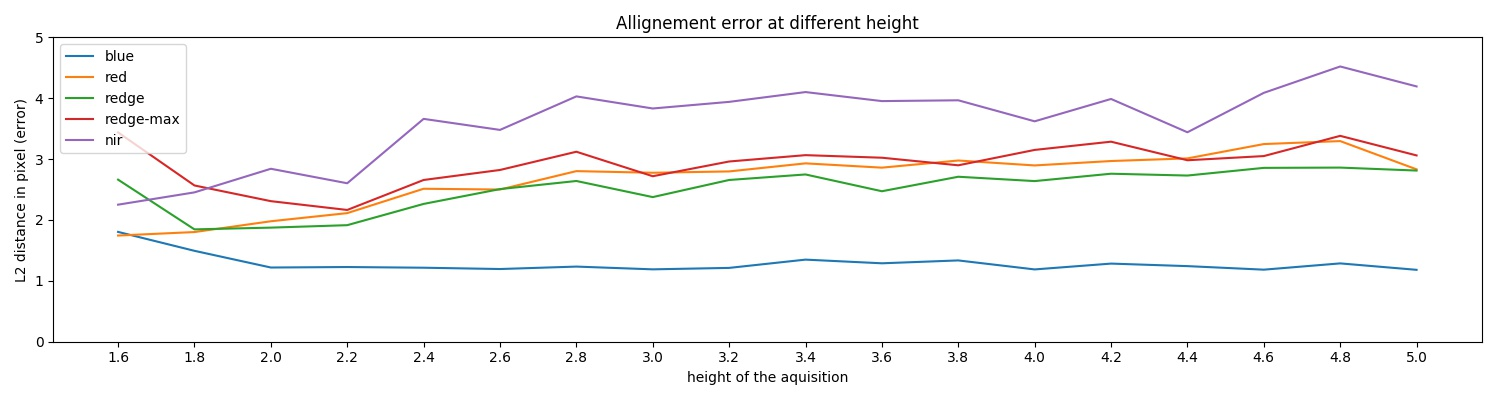
\includegraphics[width=0.8\linewidth]{../figures/affine-allignement-rmse.jpg} \\
				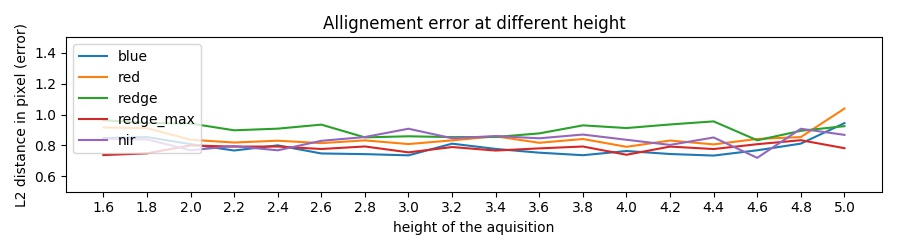
\includegraphics[width=0.8\linewidth]{../figures/prespective-allignement-rmse.jpg}
				\caption{Performance evaluation with 570nm as reference using GFTT1}
			\end{figure}
		\end{frame}
	
		\begin{frame}{Results}
			\begin{figure}
				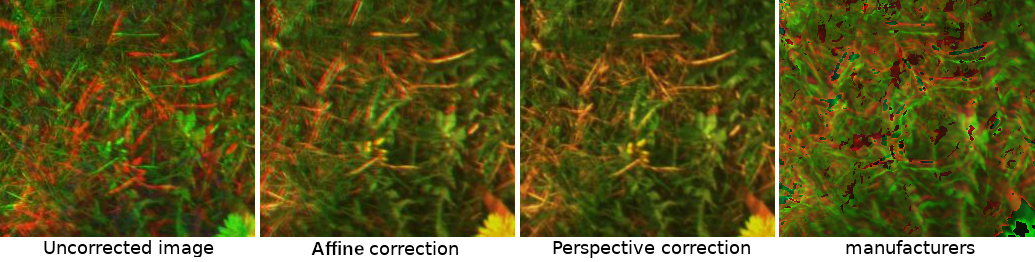
\includegraphics[width=\linewidth]{../figures/merged-correction}
				\caption{Result in pictures}
				\label{fig:affine5}
			\end{figure}
			\begin{multicols}{2}
				\begin{itemize}
					\item uncorrected $\approx 62px$
					\item manufacturer's $\approx 12px$
					\item affine $2 \approx 3px$
					\item perspective $\approx 1px$
				\end{itemize}
			\end{multicols}
		\end{frame}
	
	%\section{Discussion}
	%
	%	\begin{frame}{Discussion}
	%		This enable us to :
	%		\begin{itemize}
	%			\item Detect weed and crop
	%			\item Make image segmentation
	%			\item Extract precises features
	%		\end{itemize}
	%	\end{frame}
	
	\section{Conclusion}
	
		\begin{frame}{Conclusion}
			We have proposed a two-step method:
			\begin{itemize}
				\item A first rough correction, to get spatial properties
				\item A second full correction, using key-points
			\end{itemize}
		
			This methods is generalizable :
			\begin{itemize}
				\item Code open-source : \\ {\tiny \url{https://gitlab.com/phd-thesis-adventice/phd-airphen-alignment} }
				\item Only need two datasets using your specific camera/scene
				\item Make the calibration and extract the benchmark
				\item Use the best combination of key-points detector and reference
			\end{itemize}
		\end{frame}
	
		\begin{frame}{Conclusion}
			For our specific use, such as our camera and scene, we have determined through a benchmark:
			
			\begin{itemize}
				\item the best spectral reference are 570 and 710nm \\ (studies still define empirically 850nm).
				\item the best key-point detector is GFTT (time and number) \\ (studies still use ORG or KAZE).
			\end{itemize}
			
			Better performances than the manufacturer's (12px to 1px)
		\end{frame}
		\begin{frame}{Perspective}
			\begin{itemize}
				\item Benchmark of key-points detectors using others cameras
				\item Benchmark of key-points detectors using others scenes
				\item Study about the spatial distribution of key-points
				\item Are the best spectral bands references almost the same ?
				\item Test of different deformations models
				\item More modalities about key-points detectors parameters
				\item Optimization with more efficient matching algorithms
			\end{itemize}
		\end{frame}
	\section{Thank you for listening ! \\ Questions ?}
			
\end{document}